\documentclass[a4paper, titlepage]{article}

% For equations
\usepackage{amsmath}

% For including figures
\usepackage{graphicx}
\usepackage{float}

% Bibiliography setup
\usepackage[square]{natbib}
\bibliographystyle{agsm}
\usepackage[nottoc]{tocbibind}

% For typesetting matlab
\usepackage{listings}
\usepackage{color} %red, green, blue, yellow, cyan, magenta, black, white
\definecolor{mygreen}{RGB}{28,172,0} % color values Red, Green, Blue
\definecolor{mylilas}{RGB}{170,55,241}

\lstset{language=Matlab,%
    basicstyle=\small,
    breaklines=true,%
    frame = single,
    morekeywords={matlab2tikz},
    keywordstyle=\color{blue},%
    morekeywords=[2]{1}, keywordstyle=[2]{\color{black}},
    identifierstyle=\color{black},%
    stringstyle=\color{mylilas},
    commentstyle=\color{mygreen},%
    showstringspaces=false,
    numbers=left,%
    numberstyle={\tiny \color{black}},% size of the numbers
    numbersep=9pt, % this defines how far the numbers are from the text
    emph=[1]{for,end,break},emphstyle=[1]\color{red}, %some words to emphasise
    %emph=[2]{word1,word2}, emphstyle=[2]{style},    
}


%\title{Laboratory Work 1\\
%Coupled Drives\\
%\large EEA004}
%\author{Dan Thilderkvist, Philip Gutierrez}

\begin{document}

%\maketitle

\begin{titlepage}
  \begin{center}
    \vspace*{1cm}
    
\includegraphics[scale=1.0]{../figures/hig_logo_eng.png}\\
    \vspace{1.5cm}
    \large EEA004 - Multivariable and Nonlinear Control Systems\\
    \large Laboratory Work 1\\
    \vspace{1.5cm}
    Group 4\\
    Dan Thilderkvist and Philip Gutierrez\\
    dan.thilderkvist@hotmail.com philipgutierrez67@gmail.com\\
    Files: TBD\\
    \vspace{1cm}
    \today
  \end{center}
\end{titlepage}

\section{Introduction}
In this experiment a coupled system is decoupled and controlled.
The system studied is the control of speed and tension of a material in a continuous system.
The experiments herein is carried out using Simulink with a transfer function model based on a real experimental setup, figure \ref{fig:expSys}.

\begin{figure}[h!]
\center
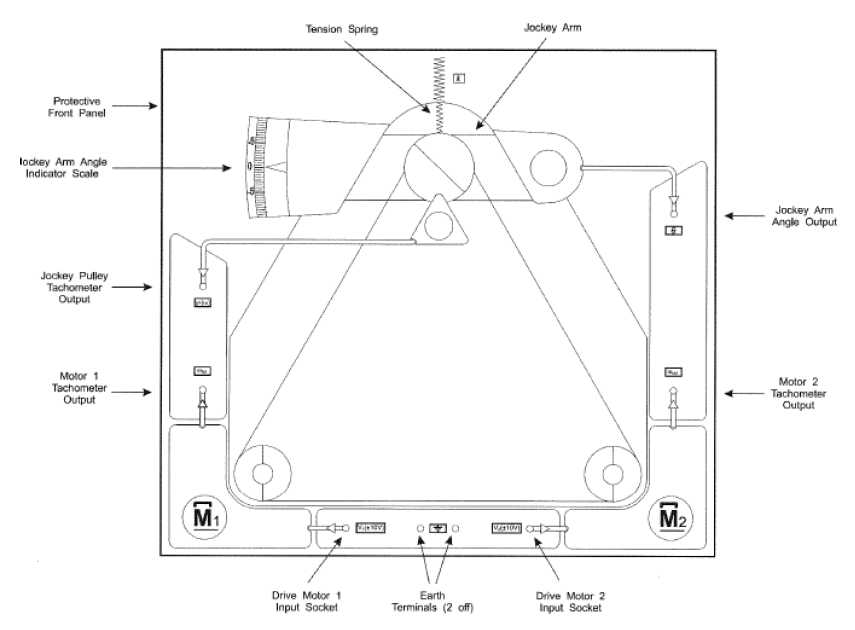
\includegraphics[scale=0.65]{../figures/experimentSystem.png}
\caption{Experimental setup that is mimicked in Simulink.}
\label{fig:expSys}
\end{figure}

The system inputs are the motor torques $u_1, u_2$ and the system outputs are the jockey pulleys speed $y_1$ and arm deflection $y_2$.
The transfer function representing this system in Simulink is:

\begin{equation}
G(s) = 
\begin{pmatrix}
\frac{0.87}{2(0.66s + 1)} & \frac{0.87}{2(0.66s + 1)} \\[6pt]
-\frac{272}{s^2 + 8.05s + 263} & \frac{272}{s^2 + 8.05s + 263}
\end{pmatrix}
\label{equ:transFunc}
\end{equation}

Throughout this report the behavior of this system will be studied, both the coupled system (\ref{equ:transFunc}) and the decoupled system that will be developed.




\section{Method}
This section describe the steps performed to carry out the experiment.

\subsection{Study the step response without decoupling}
In this first experiment the system is stimulated to showcase the coupling.
Motor 1 $u_1$ is set constant $1$ while Motor 2 $u_2$ is pulsed with square wave of period 50s ans amplitude 1.
The pulse generator start high and the resulting speed and tension of the material can be seen in figure \ref{fig:withoutDecoup}.

\subsection{Study the step response for a decoupled system}
To decouple the system a decoupling pre-compensator can be added the system.
This will take the input $u_1, u_2$ and output a modified signal $v_1, v_2$ that will be the new input to the coupled system (\ref{equ:transFunc}).
The transfer function for the pre-compensator is:

\begin{equation}
W(s) = 
\begin{pmatrix}
1 & -1 \\ 1 & 1
\end{pmatrix}
\end{equation}

Calculating the new transfer function from input $U(s)$ to output $Y(s)$ result in:

\begin{equation}
\begin{split}
\tilde{G}(s) = G(s)W(s) &= 
\begin{pmatrix}
\frac{0.87}{2(0.66s + 1)} & \frac{0.87}{2(0.66s + 1)} \\[6pt]
-\frac{272}{s^2 + 8.05s + 263} & \frac{272}{s^2 + 8.05s + 263}
\end{pmatrix}
\begin{pmatrix}
1 & -1 \\ 1 & 1
\end{pmatrix} = \\
&= \begin{pmatrix}
2\frac{0.87}{2(0.66s + 1)} & 0 \\[6pt]
0 & 2\frac{272}{s^2 + 8.05s + 263}
\end{pmatrix} = \\
&= \begin{pmatrix}
\frac{0.87}{0.66s + 1} & 0 \\[6pt]
0 & \frac{544}{s^2 + 8.05s + 263}
\end{pmatrix}
\end{split}
\label{equ:decoupled}
\end{equation}

With only elements on the diagonal, the system is now completely decoupled.
Rerunning the experiment were one input is constant ($u_1$) and the other is pulsed ($u_2$) will generate the results in figure X.
If the inputs were to be exchanged ($u_1$ pulsed, $u_2$ constant) the result is as in figure \ref{fig:withDecoupSpeed}.

\subsection{Study the decoupled system with feedback control}
Now 2 feedback PID controllers are added to the system.
One for each of the now decoupled inputs to control speed and tension independently.
For the speed system a PI controller is chosen as the system is only first order.
The closed loop system with a PI controller is then:

\begin{equation}
G_{cl} = \frac{GC}{1 + GC} = \frac{1.3182(K_ps+K_i)}{s^2 + (1.3182K_p+1.5152)s + 1.3182K_i}
\label{equ:closeLoopSpeed}
\end{equation}

This closed loop system has unity DC gain for any choice if controller gains.
It has 2 poles and one zero, the zero will increase the speed of the system slightly and increase the overshoot.
Ignoring the zero, the closed loop system can be compared to the standard model:

\begin{equation}
\frac{\omega_n^2}{s^2 + 2\zeta\omega_ns + \omega_n^2}
\end{equation}

Choosing the natural frequency and damping will allow us to design our system (\ref{equ:closeLoopSpeed}) to mimic a standard second order system apart from the effect of the zero.
Choosing the natural frequency to be 0.4Hz ($\omega_n = 0.4*2*\pi \approx 2.51rad/s$ should hopefully be quick enough.
Then choosing a damping slightly higher than 1 (due to the overshoot effect of the zero) should give a system without much overshoot.

\begin{equation}
\begin{split}
&\begin{cases}
\omega_n = 2.5 \\ \zeta = 1.2
\end{cases} \rightarrow \\
&\begin{cases}
K_i = \frac{\omega_n^2}{1.3182} = 4.7414 \\
K_p = \frac{2\zeta\omega_n - 1.5152}{1.3182} = 3.4023
\end{cases} \rightarrow \\
&C(s) = K_p + \frac{K_i}{s} = 4.7414 + \frac{3.4023}{s}
\end{split}
\end{equation}

The performance of the PI controller for speed control can be seen in figure X.

For designing the tension controller the plant equation is of second order.
To have full freedom of poles for the closed loop system the full PID controller is required.
The closed loop system will then become 3rd order with two zeros.
A third order system could be designed in the same manner as for the speed control if one pole is chosen far from the imaginary axis and the zeros are ignored.
This is however not straight forward as it require factorization and the effect of two zeros is more complex.
Instead the PID gains are tuned by trial and error by first incrementing the proportional gain, followed by integral gain and derivative gain until an acceptable performance is acquired.
This is iterated until the step response is satisfactory.
Acceptable performance is a system with similar settling time as the speed control system and minimal overshoot.
Desired performance was acquired with the following gains:

\begin{equation}
\begin{cases}
K_p = 0.1 \\ K_i = 3 \\ K_d = 0.02
\end{cases}
\end{equation}

The performance of the closed loop tension control system can be seen in figure X and figure Y.


\section{Result}
The result of the experiments are presented here as graphs
\subsection{Study the step response without decoupling}
Figure \ref{fig:withoutDecoup} show the result when $u_2$ is a square wave. 

\begin{figure}[H]
\center
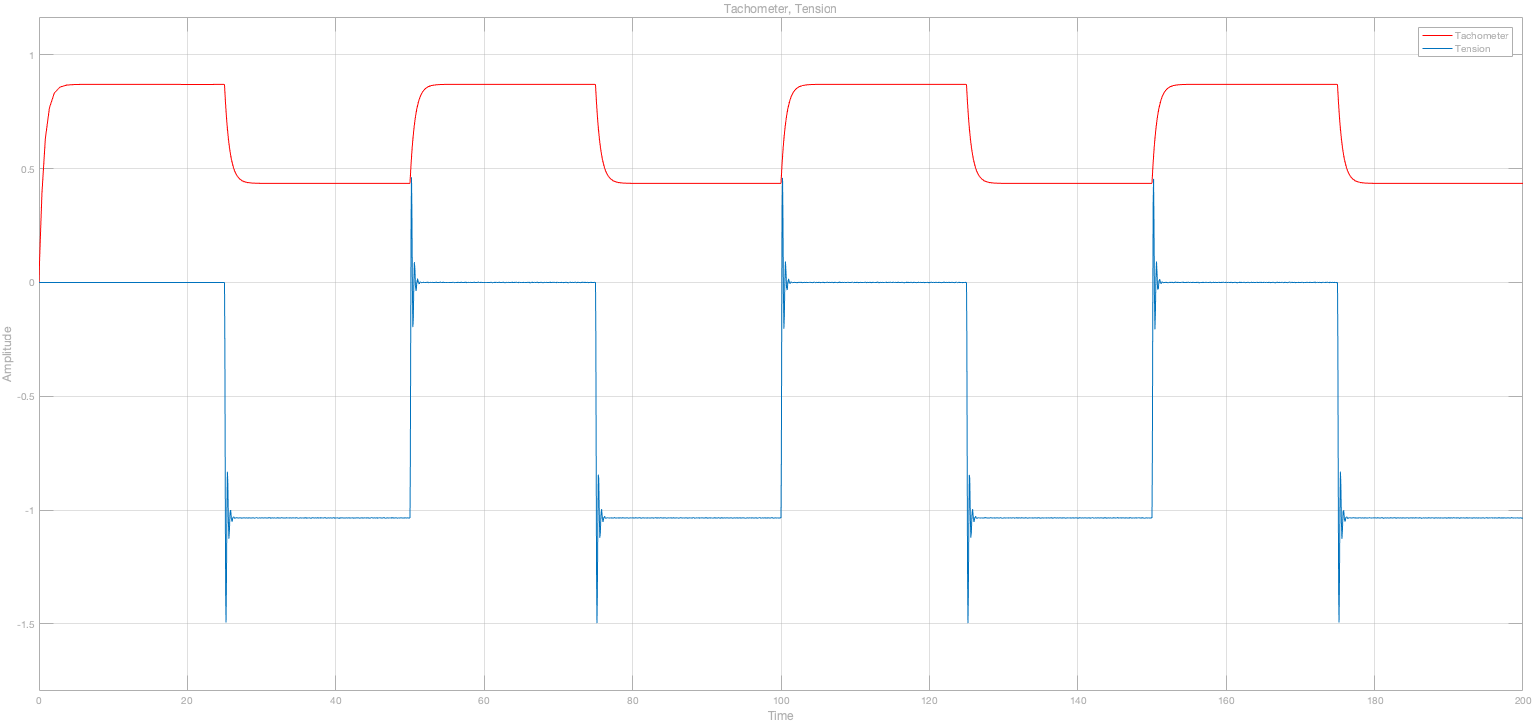
\includegraphics[scale=0.7]{../code/figures/task1.png}
\caption{Material speed and tension when holding constant $u_1 = 1$ while pulsing $u_2$.}
\label{fig:withoutDecoup}
\end{figure}


\subsection{Study the step response for a decoupled system}
Figure \ref{fig:withDecoupSpeedA} and \ref{fig:withDecoupSpeedB} show the system behavior when pulsating the decoupled inputs $u_1$ and $u_2$.

\begin{figure}[H]
\center
\includegraphics[scale=0.7]{../code/figures/task2a.png}
\caption{Material speed and tension of the decoupled system (\ref{equ:decoupled}) when holding constant $u_2 = 1$ while pulsing $u_1$.}
\label{fig:withDecoupSpeedA}
\end{figure}

\begin{figure}[H]
\center
\includegraphics[scale=0.7]{../code/figures/task2b.png}
\caption{Material speed and tension of the decoupled system (\ref{equ:decoupled}) when holding constant $u_1 = 1$ while pulsing $u_2$.}
\label{fig:withDecoupSpeedB}
\end{figure}


\subsection{Study the decoupled system with feedback control}
Here is shown how the system behaves under PID feedback control for both speed and tension.
Figure \ref{fig:withFeedbackDecoupSpeedA} show how the system behaves when pulsing the tension reference and having a constant speed reference.
Figure \ref{fig:withFeedbackDecoupSpeedB} show how the system behaves when pulsing the speed reference and having a constant tension reference.

\begin{figure}[H]
\center
\includegraphics[scale=0.7]{../code/figures/task3a.png}
\caption{PID feedback control when pulsing the tension reference with constant speed.}
\label{fig:withFeedbackDecoupSpeedA}
\end{figure}

\begin{figure}[H]
\center
\includegraphics[scale=0.7]{../code/figures/task3b.png}
\caption{PID feedback control when pulsing the speed reference with constant tension.}
\label{fig:withFeedbackDecoupSpeedB}
\end{figure}


\section{Discussion}
Figure \ref{fig:withoutDecoup} clearly show a repeating pattern in both speed and tension of period 50s.
This indicate that there is coupling from Motor 2 to both outputs.
While Motor 2 is running, both motors run at the same speed and there is no tension.
If Motor 2 is stopped (with positive direction clockwise), the tension on the material increase between Motor 1 and Motor 2 due to either the material slipping on Motor 2 or the material having to sustain the load of rotating motor 2.
The tension for the remainder of the loop will then decrease (between the jockey and the motors) and this is the measured tension output.

With the pre-compensator $W(s)$, the experiment carried out show that $u_1$ can be used to control the material speed $y_1$ and $u_2$ can be used to control the material tension $y_2$ over the jockey pulley.
This could also have been directly read out from the new transfer function $\tilde{G}(s)$ in \ref{equ:decoupled} as the elements are on the diagonal.

TODO: Another part discussing the controller result

\section{Conclusion}
TODO: Draw some basic conclusions
- Decoupling is possible for some systems by adding a pre-compensator.
- Decoupling simplifies a MIMO problem to several SISO problems



\clearpage
\bibliography{reference}

\clearpage
\appendix

\section{Example Section}
This is an example reference \citep{glad00}.

\begin{figure}[h!]
\center
%\includegraphics[scale=0.8]{../code/figures/exampleFigure.png}
\caption{Example caption.}
\label{fig:exampleLable}
\end{figure}

\lstinputlisting{../code/main.m}

\end{document}